\documentclass{article}
\usepackage{tikz} 
\usepackage[utf8]{inputenc}
\usepackage{amsmath}
\usepackage{listings}
\usepackage{amsfonts}
\usepackage{amssymb}
\usepackage{tabularx}
\usepackage{enumitem}
\usepackage{algorithm}% http://ctan.org/pkg/algorithm
\usepackage[noend]{algpseudocode}% http://ctan.org/pkg/algorithmicx
\usepackage{tikz}
\usepackage{graphicx}

\usepackage{subcaption}
\usepackage{multicol,caption}
\usepackage{geometry}
 \geometry{
 a4paper,
 total={210mm,297mm},
 left=20mm,
 right=20mm,
 top=20mm,
 bottom=20mm,
 }

\usetikzlibrary{arrows,positioning,shapes} 
\pgfarrowsdeclarecombine{ring}{ring}{}{}{o}{o}
\thispagestyle{empty}
\DeclareMathOperator{\ringarrow}{\raisebox{0.5ex}{\tikz[baseline]{\draw[ring->](0,0)--(2em,0);}}}

\tikzset{
    %Define standard arrow tip
    >=stealth',
    %Define style for boxes
    observed/.style={
           rectangle,
           rounded corners,
           draw=black, thick,
           minimum width=3em,
           minimum height=1.5em,
           font=\footnotesize,
           text centered,
           fill=blue!20!white},
     latent/.style={	
           circle,
           rounded corners,
           draw=black, thick, dashed,
           minimum width=.5em,
           minimum height=.5em,
           font=\footnotesize,
           text centered,
           fill=black!10!white
           },
    % Define arrow style
    pil/.style={
           o->,
           thick,
           shorten <=2pt,
           shorten >=2pt,},
    sh/.style={ shade, shading=axis, left color=red, right color=green,
    shading angle=45 }
    
}
   
\begin{document}
\def\ci{\perp\!\!\!\perp} % from Wikipedia



%\multicolumn{'num_cols'}{'alignment'}{'contents'}

\begin{figure}[h]
\begin{subfigure}[t]{0.45\textwidth}
\centering
\caption{Unrandomized}
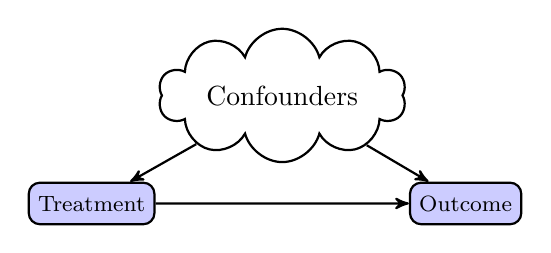
\begin{tikzpicture}[->,shorten >=0pt,shorten <=0pt,node distance=0.7cm,  thick,main node/.style={observed}, shaded/.style={latent}]
\node[cloud,draw,aspect=3](C){Confounders};
\node[main node, below left=of C](T){Treatment};
\node[main node, below right=of C](O){Outcome};
\path[]
	(C) edge (T) edge (O)
	(T) edge (O);
\end{tikzpicture}
\end{subfigure}
\begin{subfigure}[t]{0.45\textwidth}
\centering
\caption{Randomized}
\begin{tikzpicture}[->,shorten >=0pt,shorten <=0pt,node distance=0.7cm,  thick,main node/.style={observed}, shaded/.style={latent}]
\node[cloud,draw,aspect=3](C){Confounders};
\node[main node, below left=of C](T){Treatment};
\node[main node, below right=of C](O){Outcome};
\node[above left=of T](R){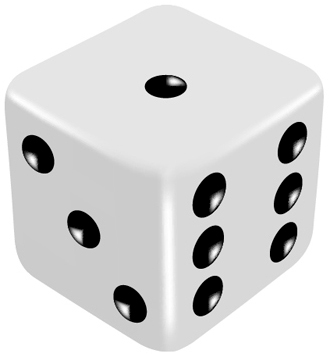
\includegraphics[width=1cm]{dice.jpg}};
\path[]
	(C) edge (O)
	(T) edge (O)
	(R) edge (T);
\end{tikzpicture}
\end{subfigure}
\end{figure}

\end{document}